\documentclass[compress]{beamer}
\usepackage{ifthen}

\setbeamertemplate{navigation symbols}{}
\setbeamertemplate{headline}{\includegraphics[height=1 cm]{../cmslogo} \hspace{0.1 cm} \includegraphics[height=1 cm]{../tamulogo} \hfill
\begin{minipage}{9 cm}
\vspace{-0.75 cm} \small
\begin{center}
\insertsection
\end{center}
\end{minipage} \hfill
\begin{minipage}{1 cm}
\vspace{-0.75 cm} \small
\begin{center}
\end{center}
\end{minipage}}

\xdefinecolor{dkred}{rgb}{0.7,0,0}
\xdefinecolor{dkblue}{rgb}{0,0,0.7}

\begin{document}
\section*{\hspace{1.5 cm} Muon Chamber Alignment\hfill Jim Pivarski}

\begin{frame}
Our goal: to develop a simple (HIP) muon alignment procedure for
\begin{center}
\begin{minipage}{0.8\linewidth}
\begin{enumerate}[\textcolor{dkblue}{(\alph{enumi})} ]
  \item 14 TeV data (expected in 2008)
  \item 0.9 TeV low-lumi data (2007)
\end{enumerate}
\end{minipage}
\end{center}

Milestones:
\begin{itemize}
  \item \textcolor{dkred}{Write muon alignment software (DONE)}
  \item \textcolor{dkred}{Demonstrate that it works (DONE)}
  \item Finalize procedure
  \begin{itemize}
    \item Data sample/cuts: \textcolor{dkblue}{(a)} $Z$ and $W$, \textcolor{dkblue}{(b)} $b\to\mu X$, beam halo
    \item Exclusion or de-weighting of muon hits in track-fit
    \item Alignment systematics: effect of backgrounds, fitting bias, \ldots
    \item Monitoring alignment quality
  \end{itemize}
  \item Full exercise with final procedure
  \item Study effect on $\sim$TeV muons from $Z'\to\mu\mu$
\end{itemize}
\end{frame}

\begin{frame}
\frametitle{Software Development}

\begin{itemize}
  \item Included muon alignables in AlignmentProducer and removed
    tracker-dependent assumptions
  \item This requred a reorganization of track refitter and
    Trajectory-calculating code
\end{itemize}
\begin{center}
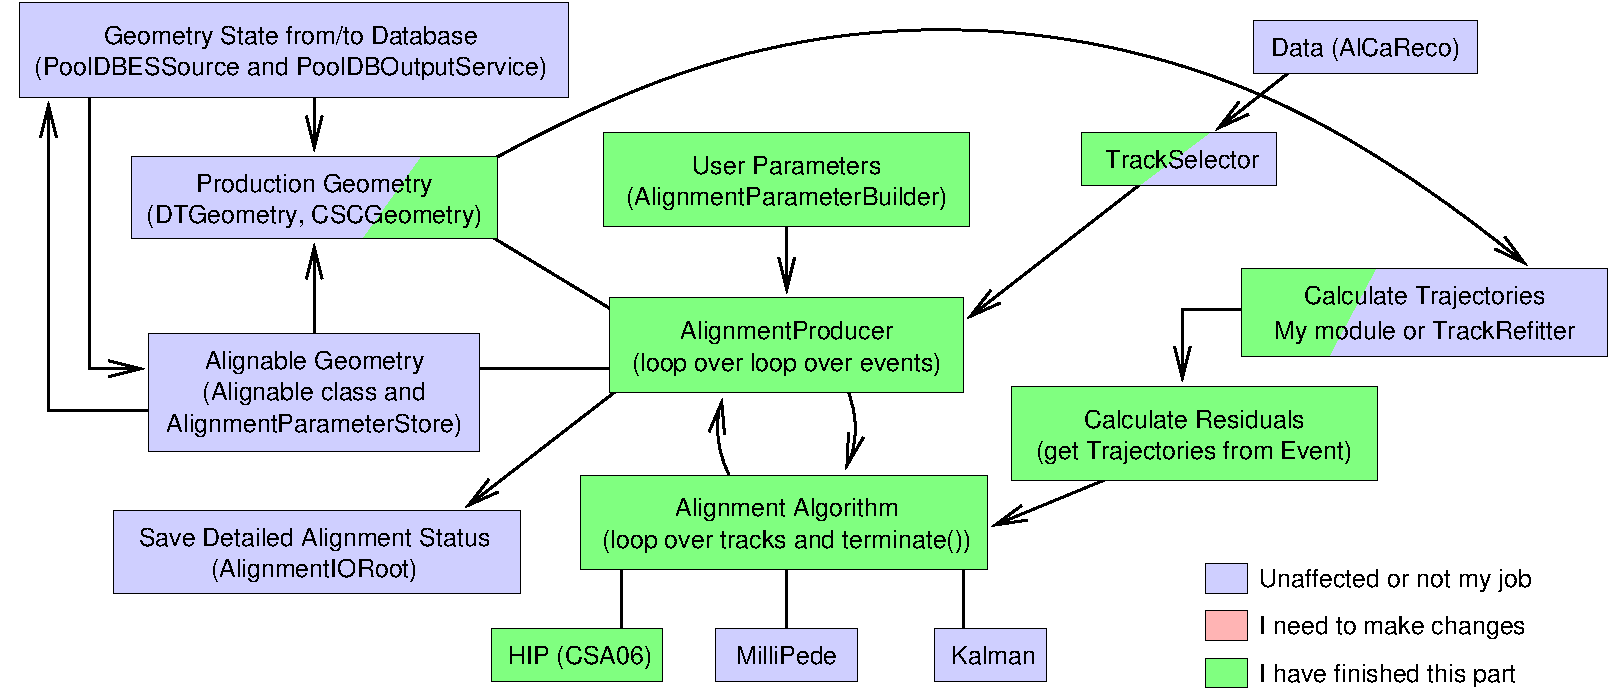
\includegraphics[width=0.75\linewidth]{flow_chart}
\end{center}

\vspace{-0.5 cm}
\begin{itemize}
  \item {\it Most} updates are in CVS
  \item We have a fully operational local copy for first alignment tests
\end{itemize}
\end{frame}

\begin{frame}
\frametitle{Corrected treatment of 1-dimensional hits}

\vfill
Our first muon alignment moved DT chambers tens of cm
\begin{itemize}
  \item CSA06AlignmentAlgorithm assumes all sensors are 2D
  \item Axial DT hits have no Z information
\end{itemize}

\vfill
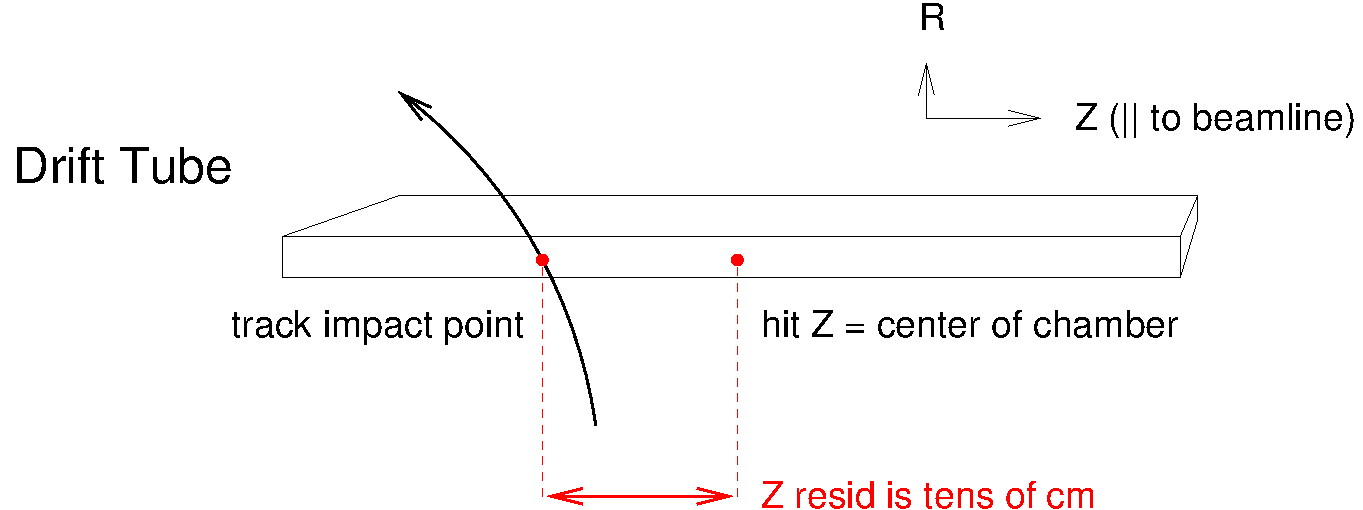
\includegraphics[width=\linewidth]{onedimhit}

\vfill
\begin{itemize}
  \item We modified the algorithm such that these hits contribute to \mbox{RPhi alignment} but not Z alignment
\end{itemize}
\end{frame}

\begin{frame}
\frametitle{First Demonstration of Muon Alignment}
\begin{tabular}{p{0.48\linewidth} p{0.48\linewidth}}
  \begin{minipage}{\linewidth}
    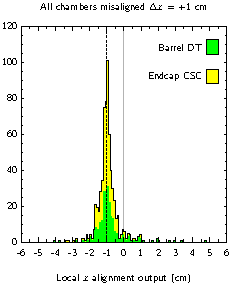
\includegraphics[width=\linewidth]{x_alignments_x_aspectratio}
  \end{minipage} &
  \begin{minipage}{\linewidth}
    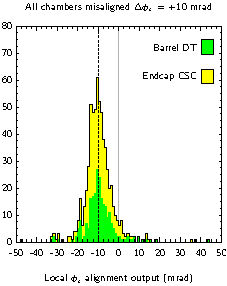
\includegraphics[width=\linewidth]{phiz_alignments_phiz_aspectratio}
  \end{minipage}
\end{tabular}

%% \begin{itemize}
%%   \item 6000 muon sample $\Rightarrow$ need 1--2 days of $Z$, $W$ for 150-300 $\mu$m
%% \end{itemize}
\end{frame}

\begin{frame}
\frametitle{Next Steps}
\begin{itemize}\setlength{\itemsep}{0.5 cm}
  \item Migrate from CSA06AlignmentAlgorithm to HIPAlignmentAlgorithm, write twiki page
  \item Define muon alignment data stream: coarse cuts for $Z\to\mu\mu$, $W\to\mu\nu$, and ``good muon''
  \item Include but de-weight muon hits in track-fit, study fitting bias
  \item Study effect of backgrounds on alignment, optimize cuts
  \item Develop a suite of quality-monitoring plots
\end{itemize}
\end{frame}

%% \begin{frame}
%% \textcolor{blue}{Goal: develop a procedure for (a) 2008 data (b) 0.9 TeV low-lumi}
%% \begin{itemize}
%%   \item Wrote muon alignment software (DONE)
%%   \begin{itemize}
%%     \item in AlignmentProducer framework (makes 3 algos available)
%%     \item using Andre's MuonAlignment interface
%%   \end{itemize}
%%   \item Develop ``final'' procedure (proof of principle is DONE)
%%   \begin{itemize}
%%     \item Include muon chambers in track-fit?  (For now, ``no.'')
%%     \item Data sample: $Z$ and $W$ for (a), low-$p_T$, beam halo for (b)
%%     \item Define event cuts (reject backgrounds) and muon track cuts
%%     \item Alignment systematics: effect of backgrounds, LS$-$OS, \ldots
%%   \end{itemize}
%%   \item Monitoring (cross-checks built into the procedure)
%%   \begin{itemize}
%%     \item Residual vs.\ everything, chamber coverage, $Z$, $W$ spectra, \ldots
%%   \end{itemize}
%%   \item Full exercise with ``final'' procedure
%%   \begin{itemize}
%%     \item Million-muon sample with backgrounds
%%     \item Define muon alignment stream for data-taking
%%     \item Read/write to database
%%   \end{itemize}
%%   \item Study effect of alignment on $\sim$TeV $Z'\to\mu\mu$
%% \end{itemize}
%% \end{frame}


\end{document}
